% Checkpoint 2: MAPPO agents on MPE2 simple_world_comm. Build: tectonic presentation/checkpoint2.tex
% Tables are generated by scripts/compare_runs.py and scripts/eval_baselines.py --agents.
\documentclass[aspectratio=169,10pt]{beamer}
\usetheme[progressbar=frametitle,numbering=fraction]{metropolis}
\usepackage[polish]{babel}
\usepackage[sfdefault,lining]{FiraSans}
\usepackage{FiraMono}
\usepackage{booktabs}
\usepackage{amsmath}
\usepackage{hyperref}
\graphicspath{{figures/}}

\title{MPE2: Simple World Comm}
\subtitle{Agenci MAPPO: trening i wyniki}
\author{Jerzy Czarnecki, Mateusz Małachowski}
\institute{Uczenie ze wzmocnieniem}
\date{}

\newcommand{\code}[1]{\texttt{#1}}

\begin{document}

\maketitle

% ---------------------------------------------------------------------------
\begin{frame}{Przypomnienie: środowisko}
  \begin{columns}[T]
    \begin{column}{0.34\textwidth}
      \centering
      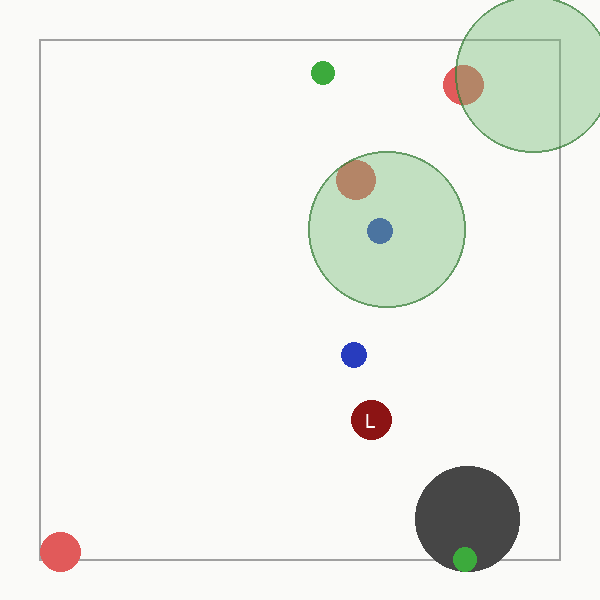
\includegraphics[width=\linewidth]{map_seed0.png}
    \end{column}
    \begin{column}{0.62\textwidth}
      \small
      \begin{itemize}
        \item 4 drapieżników (w tym lider wysyłający komunikaty) kontra 2 szybsze ofiary
        \item lasy ukrywają agentów, jedzenie daje nagrodę ofiarom
        \item epizod: 25 kroków
        \item drapieżnicy: wspólna nagroda za złapania; ofiary: kara za złapanie,
          nagroda za jedzenie, kara za wyjście z areny
      \end{itemize}
      \textbf{Cel na ten etap}: obie drużyny trenowane jednocześnie, lepsze od
      heurystycznych przeciwników
    \end{column}
  \end{columns}
\end{frame}

% ---------------------------------------------------------------------------
\begin{frame}{Algorytm: MAPPO}
  \small
  \begin{columns}[T]
    \begin{column}{0.5\textwidth}
      \textbf{Aktorzy} (polityki)
      \begin{itemize}
        \item jedna sieć na rolę: lider, drapieżnik, ofiara
        \item agenci tej samej roli dzielą wagi (+ numer agenta na wejściu)
        \item wejście: tylko własna obserwacja, więc w trakcie gry każdy działa samodzielnie
      \end{itemize}
      \textbf{Krytyk} (funkcja wartości $V$)
      \begin{itemize}
        \item jeden na drużynę
        \item \alert{MAPPO}: widzi stan globalny (192 liczby), tylko w treningu
        \item \alert{IPPO} (porównanie): widzi tylko obserwację agenta
      \end{itemize}
    \end{column}
    \begin{column}{0.46\textwidth}
      \textbf{Trening}
      \begin{itemize}
        \item self-play: obie drużyny uczą się naraz
        \item PPO z obcinaniem ($\epsilon=0{,}2$), GAE ($\gamma=0{,}99$, $\lambda=0{,}95$)
        \item 128 równoległych środowisk, każdy epizod na nowej planszy
        \item porównanie konfiguracji: 20 mln kroków ($\approx$1,7 h na CPU), 3 seedy
        \item najlepsza konfiguracja: 100 mln kroków ($\approx$8,5 h), 3 seedy
      \end{itemize}
    \end{column}
  \end{columns}
\end{frame}

% ---------------------------------------------------------------------------
\begin{frame}{Metodologia ewaluacji}
  \small
  \begin{columns}[T]
    \begin{column}{0.5\textwidth}
      \textbf{Jak oceniamy}
      \begin{itemize}
        \item każda drużyna MAPPO gra przeciwko stałym przeciwnikom: heurystycznym i losowym
        \item w trakcie treningu: co 50 iteracji, 512 epizodów
        \item ocena końcowa: 1000 epizodów na planszach nieużywanych w treningu
        \item każda konfiguracja trenowana z 3 seedami: podajemy średnią $\pm$ odch. std.
        \item dodatkowo MAPPO kontra MAPPO
      \end{itemize}
    \end{column}
    \begin{column}{0.46\textwidth}
      \textbf{Metryki}
      \begin{itemize}
        \item nagroda drużyny w epizodzie (średnia na agenta)
        \item \% epizodów ze złapaniem
        \item liczba złapań na epizod (kroki, w których drapieżnik dotyka ofiarę)
        \item ofiary: \% kroków poza areną, w lesie, na jedzeniu
        \item lider: entropia komunikatów (w bitach, maks. 2)
      \end{itemize}
    \end{column}
  \end{columns}
\end{frame}

% ---------------------------------------------------------------------------
\begin{frame}{Krzywe uczenia: 20 mln kroków (średnia z 3 seedów, pasmo = min--max)}
  \centering
  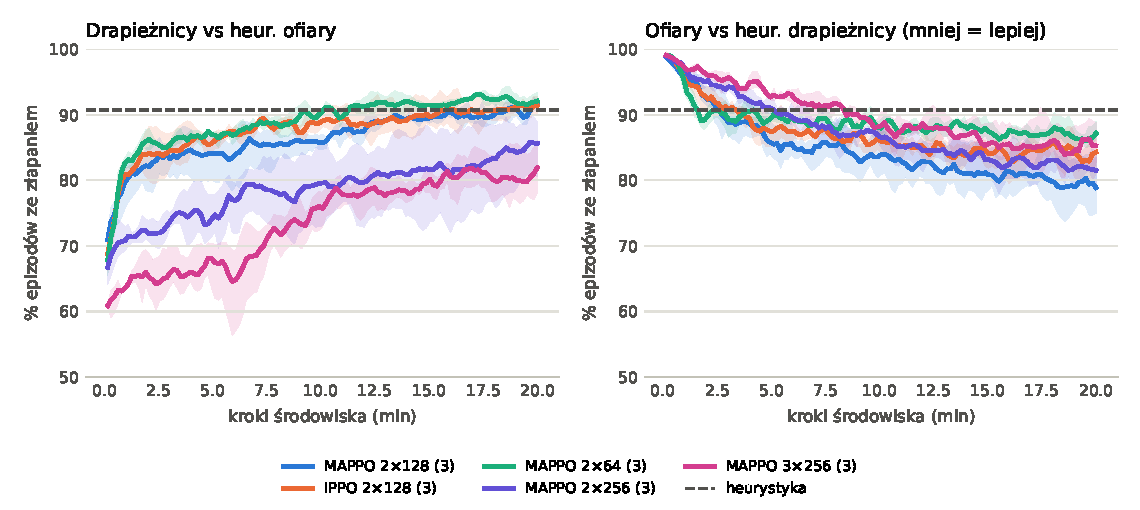
\includegraphics[width=0.92\textwidth]{compare.pdf}
\end{frame}

% ---------------------------------------------------------------------------
\begin{frame}{Porównanie konfiguracji (20 mln kroków)}
  \centering
  \scriptsize
  % generated by scripts/compare_runs.py - do not edit
\begin{tabular}{@{}lrrrr@{}}
\toprule
konfiguracja & nagr. drap. vs heur. & drap. vs heur.: złapane & ofiary vs heur.: złapane & nagr. ofiar vs heur. \\
\midrule
MAPPO 2×128 & 19,8 $\pm$ 0,8 & 91 $\pm$ 1\% & 79 $\pm$ 4\% & -8,8 $\pm$ 1,2 \\
IPPO 2×128 & 19,7 $\pm$ 1,3 & 91 $\pm$ 1\% & 84 $\pm$ 3\% & -10,2 $\pm$ 0,6 \\
MAPPO 2×64 & 21,3 $\pm$ 0,5 & 92 $\pm$ 1\% & 87 $\pm$ 1\% & -11,1 $\pm$ 0,5 \\
MAPPO 2×256 & 15,6 $\pm$ 1,1 & 86 $\pm$ 4\% & 82 $\pm$ 1\% & -9,0 $\pm$ 0,6 \\
MAPPO 3×256 & 12,4 $\pm$ 1,6 & 81 $\pm$ 3\% & 86 $\pm$ 3\% & -10,6 $\pm$ 0,8 \\
\bottomrule
\end{tabular}
\\[2pt]
  {\tiny wynik = średnia z ostatnich 5 ocen; średnia $\pm$ odch. std. z 3 seedów}\\[8pt]
  \raggedright
  \small
  \begin{itemize}
    \item heurystyka dla porównania: drapieżnicy 18,1 nagrody i 91\% złapań, ofiary złapane w 91\% epizodów
    \item najlepsze ofiary: \alert{MAPPO 2×128} (79\% złapań, heurystyczne 91\%); krytyk z
      dostępem do stanu globalnego pomaga względem IPPO (84\%)
    \item większe sieci (2×256, 3×256) uczą się wolniej i po 20 mln kroków są słabsze
  \end{itemize}
\end{frame}

% ---------------------------------------------------------------------------
\begin{frame}{MAPPO 2×128: trening do 100 mln kroków (3 seedy)}
  \centering
  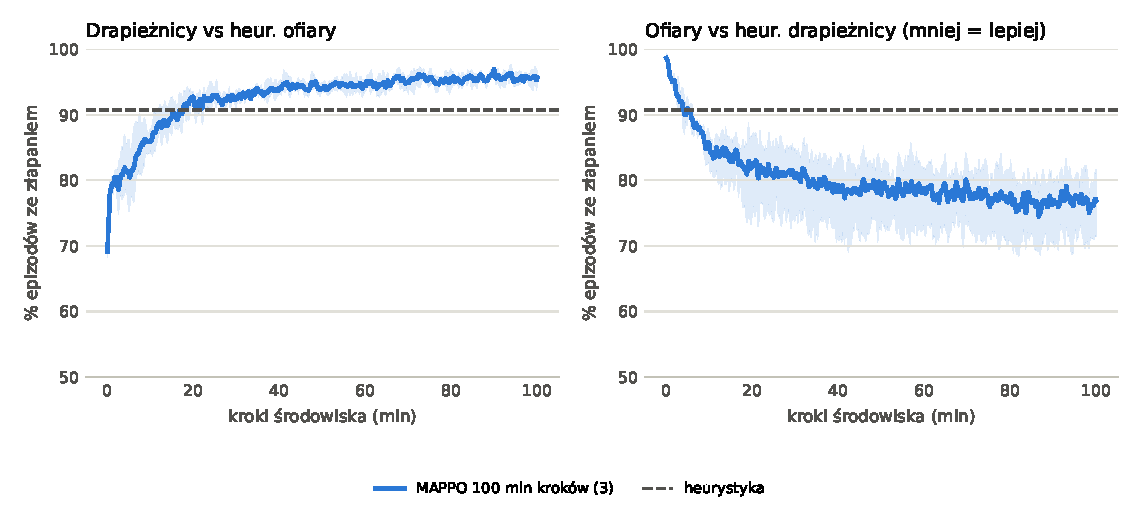
\includegraphics[width=0.86\textwidth]{long.pdf}\\[2pt]
  \raggedright
  \small
  \begin{itemize}
    \item drapieżnicy poprawiają się do końca: 91\% $\to$ 96\% złapań, nagroda 19,8 $\to$ 25,6
    \item ofiary poprawiają się głównie do $\approx$40 mln kroków: 79\% $\to$ 77\% złapań
  \end{itemize}
\end{frame}

% ---------------------------------------------------------------------------
\begin{frame}{Agenci MAPPO (100 mln kroków) kontra baseline'y}
  \centering
  \scriptsize
  % generated by scripts/eval_baselines.py - do not edit
\begin{tabular}{@{}llrrrrr@{}}
\toprule
drapieżnicy & ofiary & nagroda drap. & nagroda ofiar & złapania & epiz. ze złapaniem & ofiary poza areną \\
\midrule
heurystyczni & heurystyczni & 18,1 & -11,9 & 3,71 & 91\% & 3\% \\
MAPPO & heurystyczni & 25,8 & -17,6 & 5,18 & 96\% & 6\% \\
MAPPO & losowi & 33,6 & -42,2 & 6,43 & 96\% & 23\% \\
heurystyczni & MAPPO & 11,5 & -7,8 & 2,52 & 76\% & 1\% \\
losowi & MAPPO & 1,4 & -2,9 & 0,74 & 32\% & 0\% \\
MAPPO & MAPPO & 12,7 & -8,7 & 2,76 & 78\% & 1\% \\
\bottomrule
\end{tabular}
\\[2pt]
  {\tiny 1000 epizodów na planszach spoza treningu; wyniki MAPPO uśrednione po 3 seedach}\\[8pt]
  \raggedright
  \small
  \begin{itemize}
    \item drapieżnicy MAPPO wyraźnie lepsi od heurystycznych: 25,8 vs 18,1 nagrody, 96\% vs 91\% epizodów ze złapaniem
    \item ofiary MAPPO trudniejsze do złapania: 76\% vs 91\% epizodów, prawie nie wychodzą poza arenę
    \item MAPPO kontra MAPPO: złapanie w 78\% epizodów
  \end{itemize}
\end{frame}

% ---------------------------------------------------------------------------
\begin{frame}{Agenci MAPPO w akcji}
  \centering
  % the strip links to the video; the mp4 is played separately during the talk
  \href{run:media/mappo_agents.mp4}{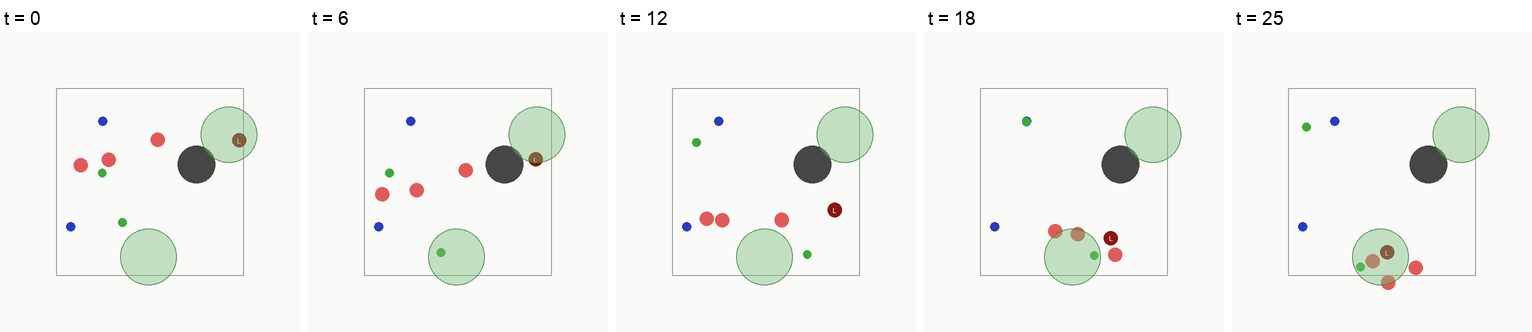
\includegraphics[width=\textwidth]{mappo_strip.png}}\\[6pt]
  \small
  \raggedright
  \begin{itemize}
    \item ofiary MAPPO przebywają w lesie w 21\% kroków (heurystyczne: 19\%), więc lasu prawie nie wykorzystują
    \item lider korzysta z różnych komunikatów (entropia 1,5 bita z maks. 2), heurystyczny lider zawsze wysyła ten sam
  \end{itemize}
\end{frame}

% ---------------------------------------------------------------------------
\begin{frame}{Różne ustawienia środowiska (trening 20 mln kroków)}
  \centering
  \scriptsize
  % generated by scripts/eval_env_settings.py - do not edit
\begin{tabular}{@{}lrrrr@{}}
\toprule
ustawienie & seedy & heur. vs heur. & drap. MAPPO vs heur. ofiary & heur. drap. vs ofiary MAPPO \\
\midrule
2 lasy, 25 kroków (domyślne) & 3 & 3,71 & 4,14 (1,12×) & 2,76 (0,74×) \\
0 lasów & 2 & 3,59 & 4,82 (1,34×) & 1,93 (0,54×) \\
4 lasy & 2 & 3,61 & 3,82 (1,06×) & 3,08 (0,85×) \\
epizod 50 kroków & 2 & 8,58 & 10,94 (1,28×) & 7,13 (0,83×) \\
\bottomrule
\end{tabular}
\\[2pt]
  {\tiny średnia liczba złapań na epizod (w nawiasie: względem heurystyki w tym samym ustawieniu); 1000 epizodów na planszach spoza treningu}\\[8pt]
  \raggedright
  \small
  \begin{itemize}
    \item im więcej lasów, tym mniejsza przewaga drapieżników MAPPO nad heurystyką: 1,34× $\to$ 1,12× $\to$ 1,06×
      (agent w lesie jest niewidoczny dla innych)
    \item bez lasów ofiary MAPPO są łapane prawie o połowę rzadziej niż heurystyczne (0,54×)
    \item trening na 50 krokach: drapieżnicy lepsi niż przy 25 krokach (1,28× vs 1,12×),
      ofiary bez poprawy i z dużą różnicą między seedami (5,3 i 9,0 złapań)
  \end{itemize}
\end{frame}

% ---------------------------------------------------------------------------
\begin{frame}{Dłuższe epizody: agenci z 25 kroków bez ponownego treningu}
  \centering
  \scriptsize
  % generated by scripts/eval_length.py - do not edit
\begin{tabular}{@{}lrrr@{}}
\toprule
długość epizodu & heurystyka vs heurystyka & drap. MAPPO vs heur. ofiary & heur. drap. vs ofiary MAPPO \\
\midrule
25 kroków & 3,71 & 5,16 (1,39×) & 2,51 (0,68×) \\
50 kroków & 8,58 & 11,61 (1,35×) & 5,39 (0,63×) \\
100 kroków & 18,32 & 24,16 (1,32×) & 11,10 (0,61×) \\
\bottomrule
\end{tabular}
\\[2pt]
  {\tiny średnia liczba złapań na epizod (w nawiasie: względem heurystyki); 1000 epizodów; agenci MAPPO po 100 mln kroków, 3 seedy}\\[8pt]
  \raggedright
  \small
  \begin{itemize}
    \item od 50 kroków prawie każdy epizod kończy się złapaniem, więc porównujemy liczbę złapań
    \item przewaga nad heurystyką się utrzymuje: drapieżnicy MAPPO łapią $\approx$1,3× częściej,
      ofiary MAPPO są łapane $\approx$0,6× tak często jak heurystyczne
  \end{itemize}
\end{frame}

% ---------------------------------------------------------------------------
\begin{frame}{Wnioski}
  \begin{itemize}
    \setlength{\itemsep}{3pt}
    \item \textbf{Obie drużyny MAPPO są lepsze od heurystyki}\\
      {\small drapieżnicy: 25,8 vs 18,1 nagrody; ofiary złapane w 76\% epizodów zamiast 91\%}
    \item \textbf{Dłuższy trening pomaga głównie drapieżnikom}\\
      {\small 20 $\to$ 100 mln kroków: drapieżnicy 91\% $\to$ 96\% złapań, ofiary 79\% $\to$ 77\%}
    \item \textbf{Krytyk ze stanem globalnym pomaga ofiarom}\\
      {\small MAPPO 79 $\pm$ 4\% złapań vs IPPO 84 $\pm$ 3\%; dla drapieżników bez różnicy (91\%)}
    \item \textbf{Większa sieć nie pomaga}\\
      {\small 2×256 i 3×256 po 20 mln kroków słabsze od 2×128; 2×64 najlepsza dla drapieżników}
    \item \textbf{Lasy utrudniają naukę}\\
      {\small przewaga drapieżników MAPPO nad heurystyką: 1,34× bez lasów, 1,06× przy 4 lasach}
    \item \textbf{Wyniki powtarzalne w domyślnym ustawieniu}\\
      {\small odchylenie między 3 seedami do kilku p.p.}
  \end{itemize}
\end{frame}

\end{document}
